\chapter{Implementation}
This chapter describes the implementation for creating a dictionary-based classifier. Several programs were made to achieve this goal, and many of the programs depends on the results from other programs. This chapter covers all the phases of the implementation in the order they were implemented. It starts by describing \emph{how to find full path of Wikipedia articles} from the Wikipedia database dump, including how to \emph{remove hidden categories} from the paths and how to \emph{handle redirects}. Further, the chapter describes the \emph{id mapping process} and compares this implementation with an implementation where full category names and article titles were used instead of ids. Deciding relevant categories is done by grading categories and category paths based on \emph{Inlink and Outlink Grading} and based on \emph{Normalized Inlink and Outlink Grading}. The mapping between Wikipedia article titles and IAB categories are described with \emph{category mapping} and with \emph{mapping between category excerpts and IAB categories}. Finally, the chapter describes the process of creating a dictionary-based classifier for other languages than English, giving an example of how to create a dictionary-based classifier for Norwegian.

\section{Finding Full Path of Articles}
\label{sec:finding_full_path_of_articles}
The goal of our implementation was to create a dictionary where the entries are created from the titles of Wikipedia articles, and each entry leads to one or more describing categories. Wikipedia already contains an underlying category structure which is useful to decide the content for each article. Thus, the first step was to find the full paths of each article in Wikipedia, where the paths are given from the categories that lead to the articles. 


% Creating a representation of the underlying structure. 

\subsection{Creating the Underlying Category Structure}
Finding full paths of all articles require information about Wikipedia's structure between categories, and between categories and articles. Thus, we needed a way of representing the available information about the Wikipedia structure. % so the relevant information could be extracted. 
The file \enwikicatlink contains the information needed to create a database table \emph{categorylinks} filled with all links between categories, all links between articles and files, and all links between categories and articles. All information about the links are inserted in the database table through \texttt{INSERT} statements where all entries are on the form\\\\
(\emph{cl\_from},\emph{cl\_to},\emph{cl\_sortkey},\emph{cl\_timestamp},\emph{cl\_sortkey\_prefix},\emph{cl\_collation},\emph{cl\_type}).\\\\
    Table \ref{tab:insertdescription} describes the meaning of all the \texttt{INSERT} statement fields \cite{wiki:categorylinkstable} and figure \ref{fig:entryexample} shows an example of an entry in a \texttt{INSERT} statement, where the link between the category with id \emph{12} and the  page \emph{Anarchism} is inserted into the table \emph{categorylinks}.  


\begin{figure}[h]
\centering
\begin{lstlisting}
(12,'Anarchism',' \nANARCHISM','2014-11-20 17:57:05',
' ','uppercase','page')
\end{lstlisting}
\caption[\texttt{INSERT} statement entry in \texttt{enwiki-latest-categorylinks.sql.gz}]{Example of an \texttt{INSERT} statement entry in \enwikicatlink. The link is between the category with id \emph{12} and the page \emph{Anarchism}.}
\label{fig:entryexample}
\end{figure}


\begin{table}[h]
\renewcommand{\arraystretch}{1.25}
\begin{tabularx}{\textwidth}{l|X}
\textbf{Entry field} &  \textbf{Description} \\ \hline
cl\_from & Stores the page.page\_id of the article where the link was placed. \\ \hline
cl\_to & Stores the name (excluding namespace prefix) of the desired category \\  \hline
cl\_sortkey & Stores the title by which the page should be sorted in a category list. \\ \hline
cl\_timestamp & Stores the time at which that link was last updated in the table. \\ \hline
cl\_sortkey\_prefix & Empty string if a page is using the default sortkey or readable version of cl\_sortkey. \\ \hline
cl\_collation & What collation is in used. \\ \hline
cl\_type & What type of article is this (file, subcat (subcategory) or page (normal page)).
\end{tabularx}
\\[10pt]
\caption[Description of entry fields in \emph{Categorylinks}]{Description of entry fields in \texttt{INSERT} statements in \emph{Categorylinks}.}
\label{tab:insertdescription}
\end{table}


\begin{figure}[h]
\begin{lstlisting}
INSERT INTO `categorylinks` VALUES 
(0,'','','2014-01-16 15:23:19','','','page'),
(10,'Redirects_from_moves','ACCESSIBLECOMPUTING','2014-10-26 04:50:23','','uppercase','page'),
(10,'Redirects_with_old_history','ACCESSIBLECOMPUTING','2010-08-26 22:38:36','','uppercase','page'),
(10,'Unprintworthy_redirects','ACCESSIBLECOMPUTING','2010-08-26 22:38:36','','uppercase','page'),
(12,'Anarchism',' \nANARCHISM','2014-11-20 17:57:05',' ','uppercase','page')
\end{lstlisting}
\caption[Excerpt from \texttt{enwiki-latest-categorylinks.sql.gz}]{Excerpt from the file \texttt{enwiki-latest-categorylinks.sql.gz} where each \texttt{INSERT} statement contains many links.}
\label{fig:categorylinks}
\end{figure}

Each \texttt{INSERT} statement consists of multiple links for insertion in the database table as we can see in figure \ref{fig:categorylinks}. The \texttt{INSERT} statements has to be split so that all links are separated into new statements, and only relevant links are kept, i.e.,  links with \emph{cl\_type} as \emph{subcat} (link between categories) or \emph{page} (link between category and article). The file \enwikicatlink contains 10 938 \texttt{INSERT} statements, which in total consists of 88 172 914 links. Table \ref{tab:enwikicatlinks} shows the number of different links found in the file. 

\begin{table}[h]
\centering
\renewcommand{\arraystretch}{1.25}
\begin{tabular}{l|l} %X}
\textbf{Links between} & \textbf{Number of links} \\ \hline
\textbf{categories} &  1 648 873\\ \hline
\textbf{categories and articles} & 21 846 996 \\ \hline
\textbf{articles and files} & 5 262 146 
\end{tabular}
\\[10pt]
\caption{Number of links found within the different link types.}
\label{tab:enwikicatlinks}
\end{table}

%A total number of #### \texttt{INSERT} statements were found in the \enwikicatlink 

%It is clear that there are lots of links within As table \ref{tab:enwikicatlinks} 

Some of the links between categories are links for maintaining the encyclopedia. The categories with this purpose are called \emph{hidden categories} and should be removed in our project in order to reduce the complexity.

\subsubsection{Hidden categories}
Wikipedia's category structure contains lots of hidden categories which are not displayed at the bottom of an article page for the general users, even if the article is placed under the category. These categories are useful for editing since it is an easy way to all mark categories with something in common, for instance mark all categories with references that needs to be checked. 

Hidden categories are concerned with maintenance and administration, hence not relevant for normal users or for our problem. The next step is therefore to remove all the links to hidden categories, which led to the task of finding all hidden categories. On Wikipedia's information page about \emph{Hidden Categories}\cite{wiki:hiddencat} are 15 385 subcategories listed as immidiate subcategories, but many of these categories have links to their own hidden subcategories which also have to be found. The first attempt was to look through all the links from the category \emph{Hidden Categories}, where 15 006 subcategories where found and marked as not relevant. Since this did not give the expected number, another attempt was made by looking at the file \texttt{enwiki-latest-page\_props.sql.gz}, where figure \ref{fig:pageprops} shows how  hidden categories are marked in the table. The next attempt was therefore to find all the ids marked with \emph{hiddencat} and find the corresponding category titles in \texttt{enwiki-latest-page.sql.gz}. This approach led to 15 513 categories. To make sure that all hidden categories where found, a test was made to see if all categories from the first attempt was found in the list created from the second attempt. The results showed that all categories found in the first attempt was also found in the second attempt, and the list of all 15 513 category titles whose links should be disregarded from further results. 

\begin{figure}[h]
\centering
\begin{lstlisting}
(747593,'hiddencat','',NULL)
\end{lstlisting}
\caption[Insert statement for hidden category]{Excerpt from the file \texttt{enwiki-latest-page\_props.sql.gz} where we can see that hidden categories are marked with \emph{hiddencat}}
\label{fig:pageprops}
\end{figure}

The hidden categories have to be removed carefully because they might be subcategories of visible categories or have visible categorise as their own subcategories. An example of this can be seen in figure \ref{fig:stevie_wonder_hidden}, where the double rounded rectangle is a hidden category, the rounded rectangle is a normal (visible) category and the rectangle is the article about \emph{Stevie Wonder}.
%Hidden categories can not be disregard
%19103360 article links, 391482 category links skipped

%An example of such a structure can be found from the categories leading to the article about the singer Stevie Wonder. 

\begin{figure}[h]
\centering
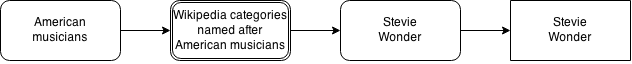
\includegraphics[width=\textwidth]{Chapters/Implementation/HiddenCategories/Stevie_wonder_hidden}
\caption[Example path with hidden category]{An excerpt of one path leading to the article about to Stevie Wonder, where the path contains a hidden category. }
\label{fig:stevie_wonder_hidden}
\end{figure}

The desirable visible paths for all articles are paths without hidden categories. The next step is therefore to change the structure so that hidden categories are removed from the structure, but without loosing any of the subcategories which might contain relevant information or  important links. Example of a how a path can be transformed is figure \ref{fig:stevie_wonder} which is the excerpt from the path in figure \ref{fig:stevie_wonder_hidden} without the hidden categories. 

\begin{figure}[h]
\centering

\includegraphics[width=.7\textwidth]{Chapters/Implementation/HiddenCategories/Stevie_wonder}
\caption[Example path without hidden category]{The desirable output of the excerpt of the path leading to the article about Stevie Wonder where the hidden category is removed from the path}
\label{fig:stevie_wonder}
\end{figure}


Table \ref{tab:withouthiddencat} shows how number of links between categories, and between categories and articles are reduced when hidden categories are not considered. 

%The main reason to reduce number of links is to reduce the complexity 

\begin{table}[h]
\centering
\begin{tabular}{l|c|c}
\textbf{Links between...} & \textbf{W/ Hidden Categories} & \textbf{W/o Hidden Categories}  \\ \hline
 \textbf{subcategories} & 1 654 758  & 1 311 275\\
 \textbf{articles and categories} & 4 241 881  & 3 152 873
\end{tabular}
\caption[Number of links without hidden categories]{Number of links removed when all hidden categories are excluded. }
\label{tab:withouthiddencat}
\end{table}

\begin{comment}
Dette må endres, for dette er feil! 
\end{comment}

\subsection{Representing the Underlying Structure}
It is important that the category names are identical at all places they occur. Wikipedia is written by volunteers from all over the worlds, and users might use different encoding depending on where they are from. Thus, both a cleaning process and a normalization process should be performed on all category names. The cleaning process is to make the category names look readable, while the normalization is a process where all words are made equal regardless of character encoding \cite[p.~26]{iirbook}.

Figure \ref{fig:withnewline} is an example of a \texttt{INSERT} statement which represents a link between the category \emph{fictional\_birds} and the subcategory \emph{ducks\textbackslash n fictional ducks}. This statement is an example of two category names that need to be processed so that they appear as \emph{ficitonal birds} and \emph{fictional ducks}. This processing  is usually called a \emph{data cleaning process} \cite{datacleaning}. The data cleaning for our purpose is converting all words to lowercase, replacing underscores with spaces and splitting up titles containing the code for newline (\emph{\textbackslash n}). Wikipedia uses the code for newline to represent how the articles should be sorted. Figure \ref{fig:fictionalbirds} shows that \emph{fictional ducks} are sorted as if it started with the word \emph{ducks}.

%The cleaning process includes converting all words to lowercase, replacing underscores with spaces and splitting up all titles containing the code for newline (\emph{\textbackslash n}). Newline is a way of representing how the articles should be sorted, figure \ref{fig:withnewline} is an example of an \texttt{INSERT} statement with newline in the title of the category, where the category should be sorted as if the title was \emph{ducks} as seen in figure \ref{fig:fictionalbirds}. Hence, the relevant part of the category title is the part after the newline, and this is the part that is considered further in the results. 
% Write something about normalization here. 

%Newline inside a category title is a way for Wikipedia to save space about the category nformation.  An example of such a statement is found in figure \ref{fig:withnewline}. 

%\footnote{TODO: insert reference: part of the insertion statement from the file \enwikicatlink} 

\begin{figure}[h]
\begin{lstlisting}
(1517681,'fictional_birds','ducks\nfictional ducks','2014-10-26 03:30:11',
'ducks','uppercase','subcat')
\end{lstlisting}
\caption[\texttt{INSERT} statement with newline]{Excerpt from \texttt{enwiki-latest-categorylinks.sql.gz} showing an \texttt{INSERT} statement including a newline character. }
\label{fig:withnewline}
\end{figure}

\begin{figure}[h]
\centering
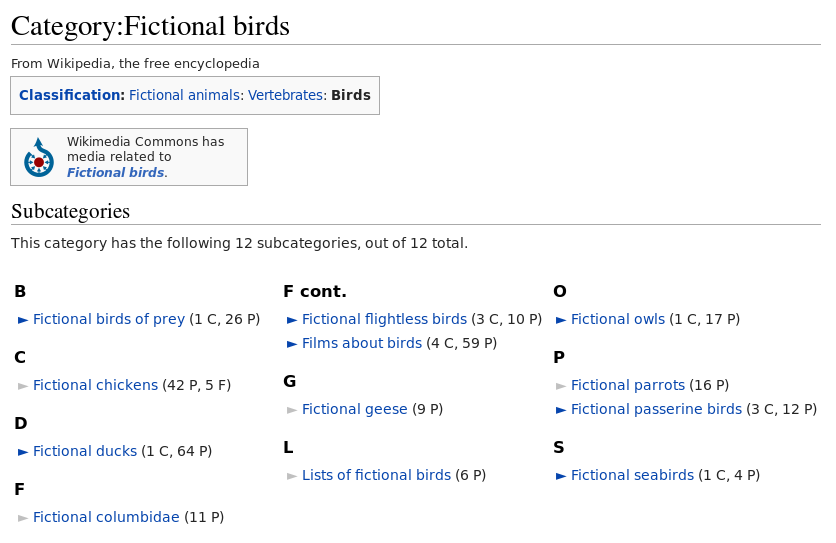
\includegraphics[width=\textwidth]{Chapters/Implementation/Fictional_birds_2}
\caption{The subcategories of the category \emph{Fictional birds} and how its subcategories are sorted based on the defined sortkey instead of the category title }
\label{fig:fictionalbirds}
\end{figure}

%This part of the \texttt{INSERT} statements means that the category \emph{fictional ducks} is both a subcategory of the category \emph{Fictional birds} and the category \emph{ducks}, hence the \texttt{INSERT} statement results in two links, one from \emph{fictional birds} to \emph{fictional ducks} and one from \emph{ducs} to \emph{fictional ducks}.

After processing all titles, they are sorted into two files depending; one for links between categories and one for links between categories and articles. These files are needed for creating the structures for finding full paths of all Wikipedia articles. 

%After the file \texttt{enwiki-latest-categorylinks.sql.gz} was split into two files where the first one contained all links between categories and the second file contained all links between categories and articles. 

\begin{comment}
\subsubsection{Creating the Category graph}
A category graph is a way of representing links between categories i.e., which categories can be reached from each category. The file containing all links between categories can be used to create such a graph. This is done by finding all subcategories of each category and removing all duplicate links. The results of this is a structure like the illustration in figure \ref{fig:catstructure}).

\begin{figure}[h]
\centering
\begin{subfigure}[b]{0.4\textwidth}
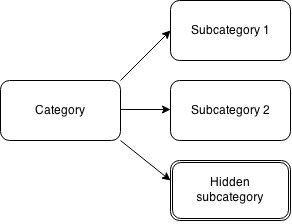
\includegraphics[width=\textwidth]{Chapters/Implementation/category-subcategories}
\caption{The structure where each category knows its subcategories}
\label{fig:catstructure}
\end{subfigure}
\begin{subfigure}[b]{0.4\textwidth}
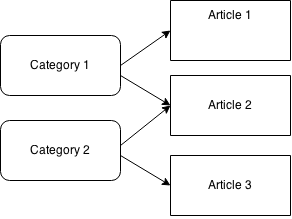
\includegraphics[width=\textwidth]{Chapters/Implementation/categories-articles}
\caption{The structure where each category know the title of its articles}
\label{fig:artstructure}
\end{subfigure}
\caption[The representation of the Wikipedia structure]{Combined this is the structure needed to represent the Wikipedia's underlying category structure as a graph}
\end{figure}


\subsubsection{Creating the Article graph}
It is also relevant to create a system of all the articles and their most describing categories, that is the categories shown at the bottom of the article page. The file containing all links between categories and their articles can be used to create a structure where each category knows its articles. Figure \ref{fig:artstructure}) illustrates this structure. 
\end{comment}
It is desirable to remove articles whose titles are not relevant for our project. Numbers without context is an example of Wikipedia article titles that are difficult to determine the meaning since a number could have various meanings, including temperatures, grades or years. Hence, all article titles which only contains numbers could be disregarded. Wikipedia contains many such articles, and a total of 23 227 articles where found. This reduces the number of links betweeen articles and categories as shown in table  \ref{tab:withoutnumber}.

\begin{table}[h]
\centering
\begin{tabular}{c|c}
\textbf{W/ Number Articles} & \textbf{W/o Number Articles}  \\ \hline
52 611 629 & 52 588 894
\end{tabular}
\caption[Number of links without number articles]{Number of links between categories and articles removed when articles only containing numbers are disregarded}
\label{tab:withoutnumber}
\end{table}


% 23227
\input{Chapters/Implementation/Articlegraph}

\subsection{Following Links Between Categories}
Finding the full paths for each Wikipedia article can be done when the representation of the structure is ready. Each path can be found by following the links between categories until an article is reached, and the links categories visited are the path. 

\begin{figure}[h]
\centering
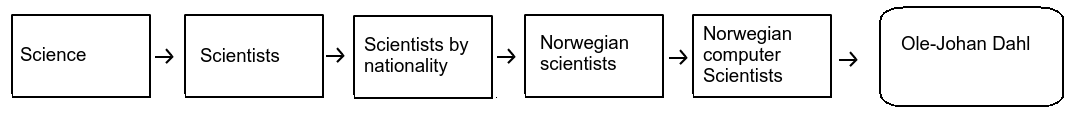
\includegraphics[width=\textwidth]{Chapters/Implementation/example_path}
\caption[Example of an article path]{Example of one of the article paths of the article \emph{Ole-Johan Dahl}. The rectangles are categories and the rectangle with rounded corners is the article. }
\label{fig:examplepath}
\end{figure}

\subsubsection{Issues with finding the full path}
The structure of Wikipedia is not represented as a tree, but as a graph. This means that there might be loops within the graph. A loop within the graph means that a category already visited in the search of a path can be reached again. Figure \ref{fig:exampleloop} shows an example of a loop in the graph. 

% 177820/907585/173722/572284/531983/173722
% people/fictional characters/fictional characters by species/fictional life forms/legendary creatures in popular culture/fictional characters by species
\begin{figure}[h]
\centering
\begin{lstlisting}
people/fictional characters/fictional characters by species/fictional life forms/legendary creatures in popular culture/fictional characters by species
\end{lstlisting}
\caption{Example of a loop found in the graph.}
\label{fig:exampleloop}
\end{figure}


This leads to problems if the program keeps going in loop and does not reach an article. A solution to this problem is to keep track on categories already visited and only follow links to categories not yet visited in the path. 
%This might mean that the path to the category is not the best one, but 

Another issue is to decide the start point for the paths, in other words the start category. Wikipedia contains some natural categories that are better to use as start categories. These categories are very general and have links to some of the major categories within different fields, hence, able to reach most other categories in the Wikipedia category structure. The category \emph{Main Topic Classifiers} was chosen for this task, because it has 22 subcategories within various fields and  where all of them have their own subcategories (see figure \ref{fig:mainclassifiers})\cite{wiki:specialtree}.

\begin{figure}[h]
\begin{center}
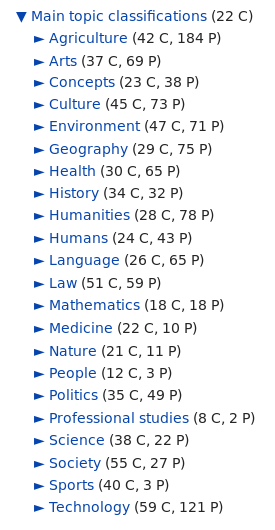
\includegraphics[width=0.48\textwidth]{Chapters/Implementation/Maintopicclassifiers.png}
\end{center}
\caption[Subcategories of \emph{Main Topic Classifiers}]{Shows the first subcategories of the chosen start category \emph{Main Topic Classifiers}. \emph{C} corresponds the the category's subcategories and \emph{P} corresponds to its pages. The figure is provided by Wikipedia's Category Tree \cite{wiki:specialtree}.}
\vspace{-20pt}
\label{fig:mainclassifiers}
\end{figure}

%The category \emph{Main Topic Classifiers} has a large variety in its subcategories which makes it possible to reach categories within many topics. 



\subsection{Irrelevant Articles and Categories}
The next step is to remove all articles that are not relevant. Some articles does not provide information and should therefore be removed from our structure to reduce number of links that have to be considered at all time. Ideally we only want to consider article titles that can provide useful information. Articles about numbers are an example of articles that does not provide any new information and can be removed. 

The full paths for an article can also be quite long, hence it is useful to reduce the complexity by removing category titles from the path that are not useful. The main reason to remove a category title from the path is if it is too specified, for instance categories that ... : 


%Some of the articles not relevant are articles which are numbers. Numbers can have many meanings, but the meaning in the Wikipedia article does not give any new information when the number is available as an entry in a dictionary. 

%\subsection{Categories not relevant for the path}
%The structure of the categories in Wikipedia are very detailed, which make many of the paths too specified for our task. To simplify the article paths are some categories therefore removed from the path. 

%The categories which where chosen to be removed where: 
\begin{itemize}
\item ... are numbers
\item ... contains number
\item ... contains the word \emph{by}
\end{itemize}

The reason to remove all categories that are or contains numbers are that they usually are connected to a specific year, which is not interesting in our case. Categories containing the words \emph{by} can usually be removed because they are a parent category for sorting categories and usually indicate what the categories are sorted by. 
%Categories containing the word \emph{by} can also be removed because the  category is usually  placed under both of the categories it represents. 
An example of this can be seen in figure \ref{fig:galileogalilei} where one of the paths found for the Italian mathematician \emph{Galileo Galilei} can be simplified. 
%which is placed under the category \emph{Italian Mathematicians by century}.

%Reducing the complexity is useful to make the paths more readable. Example of this can be showed in figure \ref{} where 

\begin{figure}
\centering
\begin{lstlisting}
/mathematics/mathematicians/italian mathematicians/italian mathematicians by century/
16th-century Italian mathematicians/galileo galilei
\end{lstlisting}
\begin{lstlisting}
/mathematics/mathematicians/italian mathematicians/galileo galilei
\end{lstlisting}

\caption[Simplification of an article path]{Simplification of one of the paths of the article about Galileo Galilei}
\label{fig:galileogalilei}
\end{figure}

%\section{Wikipedia Structure}
There are two ways of accessing Wikipedia's encyclopedic information. The first way is to look up runtime as most users do when they are looking for information. The other way is more common when the information is used by other programs and

%s, which means that the program access Wikipedia's 

The other, and most common way is to download database dumps from Wikipedia. All Wikipedia articles, images and categories are stored in a database which are accessed when a user are searching for an article online. A database dump is therefore a backup of the database which are usually stored in the case of some data is lost. \footnote{TODO: reference: en.wikipedia.ort/wiki/Database\_dump} This backup is available for anyone interested at \emph{TODO: insert link}\footnote{TODO: insert reference?}. 




A database dump is defined as the table structures which is used to get the information to load

For our purpose there are some dumps that are relevant: 


I have chosen to work on the English Wikipedia, which is the largest database in with *** articles and *** pages. 

The relevant files are: 
\begin{itemize}
\item \enwikicatlink
\item \enwikipage
\item \enwikicategory
\end{itemize}

All of these files are compressed sql-files, which means that they represent files to put information into a SQL-database. Each of the files can be used to build up a database table with insert-statements, so all the information is stored in the table. 

\enwikicatlink describes all the links between categories, which describes two different types of relationships in Wikipedia. The first relationship is between a Wikipedia article and a category, i.e the category *** points to the article. The other relationship is between two categories which means that one of the categories is a subcategory of the other category. 

The file contains the table "categorylinks". Since the file is quite large (1.5GB compressed), it is desirable to split the file into two files; files containing information of the relationships between categories and files that contain information about the relationship between categories and pages. 

%\section{Parsing through the dumps}
This was solved by creation the program. The program takes the \enwikicatlink as input, and goes through each INSERT-statement in the file. Since all INSERT statements contains information about many relationships, the statements are split to represent one relationship at the time. Then the statement is sorted into "Link between two categories" or "Link between a category and a page" depending on the output of the relationship described in the statement. 

Some of the information about the relationships between categories are not relevant for this problem, for instance information about hidden categories like "Unprinthworthy categories". This categories are removed in the process to reduce the number of category elements considered in the later programs. 

Wikipedia also contains lots of information about redirecting between categories and pages, for instance are article names in plural redirected to the article name in singular.  This information is also stored in \enwikicatlink and is sorted out during the process to be considered later in the process where it is desirable to redirect in the same way, but still not relevant in the early steps of the programming. 

%Category graph builder
One of the output files of the \catlinkprogram is a file containing all relationships between categories. The next step is to sort this information so that a category knows all its subcategories. The program \catgraphbuilderprogram takes the category information as output and creates a structure to represent the information. The output of the program is a file where all parents to a subcategory is stored. %This program should maybe consider loops as well
The program sorts all the categories and output a file where all subcategories of a category is listed under the name of their parent category.

\enwikicatlink also contains some shortcuts for saving space when information about the categories are inserted into the database. An example of such a statement is \footnote{TODO: insert reference: part of the insertion statement from the file \enwikicatlink}: 

\begin{code}
1517681,'fictional_birds','ducks\nfictional ducks','2014-10-26 03:30:11',
'ducks','uppercase','subcat' 
\end{code}

This part of the insertion statements means that the category \emph{fictional ducks} is both a subcategory of the category \emph{Fictional birds} and the category \emph{ducks}. This means that this statement has to result in the following information: 
\begin{code}
Fictional birds: 
* fictional ducks

ducks:
* fictional ducks
\end{code}

One of the problem in the results of the program is that there are potential for loops within the structure. This is because a category may be subcategory of a category, but also the parent category of the same category's parent. This means that the whole structure cannot be represented as a three, but is rather a graph where the connected categories are linked together. 

The other output file of \catlinkprogram is a file where the each line represents an article its immediately closest categories, these categories are the same as those represented at the bottom of the article page. 

It is desirable to get each article's full path for our problem. The next program made is therefore a program that takes creates an output where all articles and their immediate closest categories are stored. Here is also some cleaning done so that all categories which contains the words \emph{Wikipedia} or \emph{category} are removed since these are part of the hidden structure for sorting and not relevant for our task. 

To create the full path of each article are there 

the category graph and all the articles with it's 


%Article builder
After all category links are split into list describing relationships between categories and relationships between articles and their subcategories 


\section{Redirects}
%Wikipedia contains lots of redirects between articles to help the users find the articles they look for, and to keep the encyclopedia well-structured.  
Wikipedia contains lots of redirects to articles for two main reasons. The first is to help users find the articles they are looking for, and the second reason is to keep the encyclopedia well-structured. The redirects are divided into different types depending on the reason for redirecting. Wikipedia lists all the different reasons of redirects. \cite{wiki:redirect} 
\begin{itemize}[noitemsep]
\item[-] Alternative names 
\item[-] Plurals 
\item[-] Closely related words 
\item[-] Adjectives/Adverbs point to noun forms 
\item[-] Less specific forms of names, for which the article subject is still the primary topic. 
\item[-] More specific forms of names 
\item[-] Abbreviations and initialisms 
\item[-] Alternative spellings or punctuation
\item[-] Punctuation issues—titles containing dashes should have redirects using hyphens.
\item[-] Representations using ASCII characters, that is, common transliterations 
\item[-] Likely misspellings
\item[-] Likely alternative capitalizations 
\item[-] To comply with the maintenance of nontrivial edit history
\item[-] Sub-topics or other topics which are described or listed within a wider article
\item[-] Redirects to disambiguation pages which do not contain "(disambiguation)" in the title
\item[-] Shortcuts
\item[-] Old-style CamelCase links 
\item[-] Links auto-generated from Exif information 
\item[-] Finding what links to a section, when links are made to the redirect rather than the section.
\end{itemize}

Most of the redirect pages are places in categories which tells the reason for the redirection. The category types for the classification are \emph{Maintenance}, \emph{Visual} or \emph{Discussion}.

%When a page is marked as a redirect page in 
\subsubsection{Handling redirects}

If a page is supposed to be redirected to another page, this is found in \texttt{enwiki- latest-page.sql.gz} where the page's \texttt{INSERT} statement is marked with '1' in the 6th position if it's redirecting (see figure \ref{fig:isredirect}).

\begin{figure}[h]
\centering
\begin{lstlisting}
(10,0,'AccessibleComputing','',0,1,0,0.33167112649574004,
'20150111235554','20150112004211',631144794,69,NULL)
\end{lstlisting}
\caption{Example of a redirecting \texttt{INSERT} statement}
\label{fig:isredirect}
\end{figure}
The first attempt of handling redirects is to make sure the paths are found to articles with correct names and not to the redirecting pages. Finding all paths to pages that redirect to other pages is unnecessary and creates more data than needed. It is instead better to find all pages that other pages redirect \emph{to}. This can be found in a separate file \texttt{enwiki-latest-redirects.sql.gz} where both page id and page title for all pages are found. After all of these ids and titles are collected, the next step is to connect them with the correct output. As an example would the article from figure \ref{fig:isredirect} be connected to the page title in figure \ref{fig:correctacccomp} after the title is converted to lowercase and underscores are removed. 

\begin{figure}[h]
\centering
\begin{lstlisting}
(10,0,'Computer_accessibility','','')
\end{lstlisting}
\caption[Example of a page redirecting to]{The page title \emph{AccessibleComputing} (figure \ref{fig:isredirect}) redirect to \emph{Computer Accessibility}.}
\label{fig:correctacccomp}
\end{figure}

%Trenger at alle artiklene er lagret med de riktige navnene! 


%
%The next step in our problem is to decide which of the redirects that are relevant. 
%If the page is redirecting 
%All redirect pages are found in a separate file 

%Most redirect pages are not placed in article categories. There are three types of redirect categorization that are helpful and useful:

%    Maintenance categories are in use for particular types of redirects, such as Category:Redirects from initialisms, in which a redirect page may be sorted using the {{R from initialism}} template. One major use of these categories is to determine which redirects are fit for inclusion in a printed subset of Wikipedia. See Wikipedia:Template messages/Redirect pages for a full alphabetical list of these templates. A brief functional list of redirect category (Rcat) templates is found at {{R template index}}.
%    Sometimes a redirect is placed in an article category because the form of the redirected title is more appropriate to the context of that category, e.g. Shirley Temple Black. (Redirects appear in italics in category listings.)
%    Discussion pages. If a discussion/talk page exists for a redirect, please ensure (1) that the talk page's projects are all tagged with the "class=Redirect" parameter and (2) that the talk page is tagged at the TOP with the {{talk page of redirect}} template. If the discussion page is a redirect, then it can also be tagged with appropriate Rcats.


\section{Id Mapping}
When writing all the results to file, these files are extremely large. All path to all Wikipedia articles ended with about 20 GB compressed data of text. The result was to create a id mapping for each category name and article name. All names get a unique id, and instead of writing the full path to file, the ids of the full path is written to file. 


Another reasoning for id mapping is to make faster is that the ids are smaller than the full category names, which makes the lookups faster. 



% Sammenlikning mellom finne alle pather med id vs med navn

% Fordel 2: Kan bruke "/" in the text. 

The id mapping is fixed by creating a counter that assigns numbers to each category name or article name that is not found yet.  

\section{Grading of Categories}

\begin{comment}
The structure of Wikipedia could be considered confusing since anyone can edit. This means that the underlying category structure of Wikipedia contains lots of links between all categories. 

This means that it is possible to reach almost all articles from each category. 

This means that there are categories that reach lots of other categories. These should not be considered as important as the other categories. A program was made to find these categories. 

There are 28 top categories (direct subcategories of %\emph{Main Topic Classifications}). 

The main assumption is that if a category leads to many of the top categories, it is possible to reach lots of articles which are not associated with the category. 

%\begin{code}
Eksempel på hvordan kategorier finner artikler som ikke har noen sammenheng med kategorien.
%\end{code}

If a category leads to many of these 
The top categories (28) leads to lots of subcategories. 

% Fan
Another way of finding categories that does not provide information about the path, is to find all categories with many parent categories and with many subcategories since this means that they easily can reach categories not relevant for the category. 

Hence a program was made to find the number of parent categories and subcategories for each category. 
\end{comment}

Many articles can be reached from categories that are not describing of the content at all, for instance is the article about \emph{Ole-Johan Dahl} (the Norwegian programmer) found from links from the category \emph{people}, but also found from links from the categories \emph{politics} and \emph{arts} (see Figure \ref{fig:olejohandahl_paths}). When all paths are found for all Wikipedia articles, the next step was to grade each path depending on how well they describe the article. 

%grade the paths to find the paths most helpful for describing the article's content. 

\begin{figure}[h]
\centering
\begin{lstlisting}
ole-johan dahl:
*people/people categories by parameter/categories by nationality/academics by nationality/norwegian academics/faculty by university or college in norway/university of oslo faculty

[...]

*politics/political activism/leadership/management/quality/software quality/formal methods/formal methods people

[...]

*arts/aesthetics/design/software design/data modeling/formal methods/formal methods people

\end{lstlisting}
\caption[Example of variety in article paths]{Some of the paths for the article about \emph{Ole-Johan Dahl}.}
\label{fig:olejohandahl_paths}
\end{figure}


\subsection{Grading based on Inlinks and Outlinks} % eller: Grading based on inlink and outlinks 
\subsubsection{Inlinks and Outlinks of Categories}
Each category in Wikipedia has a set of parent categories i.e., categories that lead to the current category, and a set of subcategories i.e., categories that can be reached from the current category. The size of these sets for a given category can be notated as 
\begin{itemize}
\item \emph{Inlink} = number of parent categories
\item \emph{Outlink} = number of subcategories
\end{itemize}
Figure \ref{fig:Categorywparentandsub} is a demonstration of how  \emph{inlink} and \emph{outlink} are connected to a category, and gives the idea that a catgory with high \emph{inlink} and \emph{outlink} are more likely to be visited when looking for paths for an article. 
\begin{figure}[h]
\centering
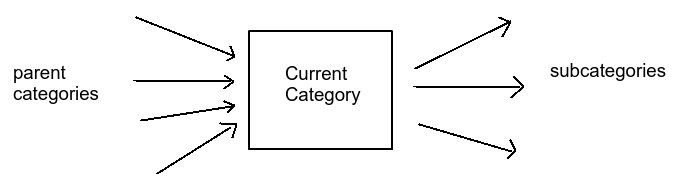
\includegraphics[width=\textwidth]{Chapters/Implementation/Grading/category_parent_sub}
\caption[Example of \emph{inlink} and \emph{outlink} for a category]{Example of how a category has links from parent categories and links to its subcategories. \emph{inlink} for the category is 4 and \emph{outlink} for the category is 3.}
\label{fig:Categorywparentandsub}
\end{figure}


The first assumption is that categories with high \emph{inlink} can be reached from categories that are not about the same. 

%great rift valley: 5, 31
\begin{figure}[h]
\centering
\begin{lstlisting}
INSERT EXAMPLE HERE: 
\end{lstlisting}
\caption{Caption}
\label{fig:my_label}
\end{figure}


\begin{figure}[h]
\centering
\begin{lstlisting}
ole-johan dahl:
*politics/political activism/leadership/management/quality/software quality/formal methods/formal methods people
\end{lstlisting}
\caption{Example of how \emph{politics} can reach the article about \emph{Ole-Johan Dahl}}
\label{fig:politicstosoftware}
\end{figure}
%quality: 9, 3
%management: 31, 5
The next assumption is that categories with a high number for \emph{outlink} are more likely to reach categories not relevant since they can reach far in all the subcategories' directions. Figure \ref{fig:politicstosoftware} shows how the Wikipedia article about \emph{Ole-Johan Dahl} can be reached from the category \emph{politics}. One of the categories with a high \emph{outlink} is the category \emph{management}, which has \emph{outlink} as 31 and hence be reached many categories. 

\subsubsection{Grading based on Inlinks and Outlinks}
The assumption that categories with high \emph{inlink} and \emph{outlink} are more often visited leads to the thought that these categories should have a lower score than categories that are more rarly visited. 

The first approach was therefore to find the \emph{inlink} and \emph{outlink} of all categories in the structure. These numbers had to be compared with the average number of \emph{inlink} and \emph{outlink} to know whether the number is high or low (see Table \ref{tab:avginlinkoutlink}). 

\begin{table}[h]
\centering
\begin{tabular}{c|c}
\textbf{Average number of \emph{inlink}} & \textbf{Average number of \emph{outlink}}\\ \hline
 5 & 2 \\
\end{tabular}
\caption{Average number of inlink and outlink}
\label{tab:avginlinkoutlink}
\end{table}

The score for each category was then 

\begin{equation} \label{eq:scoreinout}
Score_{C} = \frac{inlink_{c} + outlink_{c}}{\bar{C_{in}} + \bar{C_{out}}}
\end{equation}
where $\bar{C_{in}}$ is the average \emph{inlink} and $\bar{C_{out}}$ is the average \emph{outlink}.

The scoring from formula \ref{eq:scoreinout} means that paths with categories rarely visited will be favoured, hence given a lower score. 

\subsubsection{Evaluation of the scores}
None of the categories can have a score of 0 since this means they cannot be reached or reach other categories. The lowest score found was 0.376010, which was given to all categories with only one parent and zero subcategories, a total of 104,471 categories.  The category with the highest score is the category \emph{Albums by Artist}, which is the category with most subcategories (17,393), hence a score of $6,512.120784$. Hence the range of the scores is <0.376010, 6,512.120784> where all category scores lie within this range. 

Figure \ref{fig:scorevalue} shows how many categories are found for each of the possible score values. The figure shows that there are many categories with a low score value, while there are only a few categories for the higher score value. The categories with high score value will have a high impact on the article path, hence the path will have a smaller chance of being chosen.

\begin{figure}[h]
\centering
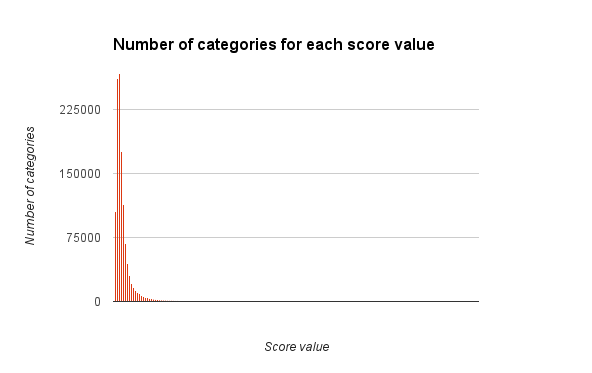
\includegraphics[width=\textwidth]{Chapters/Implementation/Grading/Inlinkoutlink_scorevalue_numberofcategories}
\caption{Number of categories for each possible score value}
\label{fig:scorevalue}
\end{figure}

%This means that the score for all categories are between 0.376010 and 6512.120784.

%This means that the scores for all categories are in the range of 0 and

%Maxgrade: 6512.120784 (albums by artist)
%Mingrade: 0.376010 (user bho-4)
\subsection{Problems with the simplified grader}
Since it is desirable with the lowest score as possible, the first problem encountered was that the program favoured short paths. 

\begin{figure}
\centering
\begin{lstlisting}
argentines of serb descent:
* society/ethnicity/ethnicity stubs/ (34.592939)
* culture/ethnicity/ethnicity stubs/ (29.704807)
* humans/ethnic groups/ethnology/ethnicity stubs/ (27.824755)
\end{lstlisting}
\caption{Caption}
\label{fig:my_label}
\end{figure}

This is both correct and wrong at the same time. It is desirable to find short paths, but there should be some punishment if the path is too short?

\begin{comment}
Problem med Alexander Huges: han er fotballspiller og dette kommer ikke så godt fra. 

asd.,kas.kdfj
\end{comment}


\begin{figure}[h]
\centering
\begin{lstlisting}
alexander hughes:
*health/health by city/health in edinburgh/sport in edinburgh/sports teams in edinburgh/football clubs in edinburgh/heart of midlothian f.c./heart of midlothian f.c. players (37.22501)
*nature/life/births by year/year of birth missing (28.576777)
*people/people categories by parameter/people by time/births by year/year of birth missing (28.200766)
\end{lstlisting}

\caption{Caption}
\label{fig:alexanderhughes}
\end{figure}

\subsection{Advanced grading based in Inlinks and Outlinks}
\subsection{Disambiguation Grading}

\section{Mapping to Desirable Output Categories}
Our goal for the mapping process is to create a link between Wikipedia article titles and one or more categories from the desirable output categories. It is essential to know the meaning of the WIkipedia rticles in order to create sucha mapping. Our theory is that this information can be found in the full paths of the articles, where a 
%, the next step is to create a link between all Wikipedia categories and the desirable categories. 
full path of a Wikipedia article contains the categories visited to reach the article. This means that the  machine needs some predefined knowledge to identify the meaning of the paths. Two approaches were tried for this task; creating a mapping between Wikipedia categories and output categories, and creating mapping between path excerpts and output categories. 

%the first was to create a mapping between the Wikipedia categories and a category from the set of output categories and the second approach was to 
%knowing the meaning of the categories is important to understand the meaning of the article. 
%\subsection{Mapping Wikipedia Categories to Desirable Output Categories}
\subsection{Deciding Output Categories based on Wikipedia Categories}
%The first step is to decide the output categories. %in other word what categories
The first approach was to create a mapping between each Wikipedia category and one or more categories in the desirable output category set. The idea was that a matching could be performed by matching Wikipedia category names and a output category name. The task of mapping each Wikiepedia category to desirable output categories is too big to be done manually since the Wikipedia category set contains 1 201 373 categories. This means that the process should be automated. One way of doing this is by looking at similarities in the words contained in the Wikipedia category and in the output category.

\subsubsection{Expanding the IAB category}
The categories in the IAB taxonomy were chosen as the desirable output category set for our task. This taxonomy  only consists of two category layers, which are not specified enough for creating a matching based on the category names. Hence the IAB taxonomy was extended with a third and more specified layer to improve the category mapping process. 

%was added to the taxonomy to 
%had to be created for this task, where this layer is specified 
%we want to classify all the Wikipedia categories to. The categories in the IAB taxonomy is not specified enough to categorize all the categories, hence it is necessary to add a third layer to the taxonomy. This layer has to be more specified to make it easier to categorize all the Wikipedia categories. 
%The next layer has to be modified to 

%fit the set of Wikipedia categories, and to be helpful for categorizing correct. 

This third layer can be viewed as common knowledge given to the machine. The second layer \emph{Europe} is an example of a layer where the machine lacks common knowledge since it does not know what countries are part of Europe. Expansion of this tier could be creating a third tier containing all European countries, which means that all Wikipedia categories containing a name of an European country should map to the category \emph{Europe}.

%An example of an expansion to the second layer \emph{Europe} is to add all European countries to its third layer since the machine lacks common knowledge about what countries 

%Such a layer can be viewed as giving the machine common knowledge. An example of 

%One of the second layers in the IAB taxonomy is \emph{Europe} under the first layer \emph{Travel}. The computer lacks common knowledge about what countries are in Europe, hence some information has to be provided to this layer so it can recognize countries in Europe. One way of doing this is by adding all European countries to a third layer under the category \emph{Europe}. 

%Since the task is categorization of Wikipedia, knowledge has been provided from other sources. List of all countries where found from \url{http://www.internetworldstats.com/list1.htm}. 

\subsubsection{Lemmatization}
%The set cof Wikipedia categories contains of 
%Our set of Wikipedia categories contains 1 201 373 categories. 

Figure \ref{fig:catmapping_exactmatch} shows how a matching between Wikipedia categories and output categories, where the output category name \emph{sports} are found as a word in the Wikipedia category name \emph{ministry of yougth affaris and sports}.

\begin{figure}[h]
\centering
\begin{lstlisting}
ministry of youth affairs and sports
sports
\end{lstlisting}
\caption[Exact match on mapping between Wikipedia category and output category]{Exact match on mapping between Wikipedia category and output category, where the output category is found in the Wikipedia category.}
\label{fig:catmapping_exactmatch}
\end{figure}
The problem with this approach is that words like \emph{sport} will not be an exact match of the word \emph{sports}, hence this Wikipedia category will not be included under the desirable output category. The next step is therefore to find matches between the categories regardless of the declension of the word. This part is called lemmatization and is defined as the process where different inflected forms of a word are grouped together \cite{wiki:lemmatisation}\cite[p.~30-33]{iirbook}. There are various lists for lemmatization available online, and a list was chosen from  \url{http://www.lexiconista.com/datasets/lemmatization/} which provided a list of common lemmatization. Both the words in the Wikipedia categories and the desirable output categories were processed by reading the lemmatization file and checked whether the words could be reduced. Figure \ref{fig:catmapping_lemmamatch} shows example of a match found after lemmatization is performed. 

\begin{figure}[h]
\centering
\begin{lstlisting}
sailors at the 1956 summer olympics
*olympics
*sailing
\end{lstlisting}
\caption[Example of match after lemmatization]{Example of a match between Wikipedia category and output category after lemmatization, where \emph{sailors} match with \emph{sailing}}
\label{fig:catmapping_lemmamatch}
\end{figure}

\begin{comment}
\subsubsection{Categories not relevant for classification}
Not all categories are suitable for classification, some categories are still just relevant for maintaining a well-structured encyclopedia. Example of such categories are \emph{container categories}, which are categories only containing subcategories. All container categories where found by looking at the file asdfasdf  . Some of these categories have already been removed because they are also hidden categories, but a total of 69 023 categories could be disregarded for this purpose. 
%Lots of categories are associated with years, but not 
%The next step was to mark all categories associated with years. These categories usually are  
\end{comment}

\subsubsection{Evaluation of Mapping Wikipedia Categories to Output Categories}
The results from this approach were not so good for two main reasons. 
%The results from this approach from this approach were not good for two main reasons: 
The first reason is that it is difficult to perform matching based on words. A perfect result could only be achieved if the computer knows all synonyms, inflections and the true meaning of all words. 

The other problem was with ambiguous words in the category names. An example of this is the categories shown in figure \ref{fig:ambiguous_category_name} where both categories contain the word \emph{Cicero}, but where the first category is for the suburb of Illinois and the other is for the Roman philosopher. Creating mapping rules for these names would be a difficult task. 

\begin{figure}[h]
\centering
\begin{lstlisting}
Category:Cicero, Illinois
Category:Cicero
\end{lstlisting}
\caption{Example of two category names which contains the same word with different meaning, and should be classified to different categories.}
\label{fig:ambiguous_category_name}
\end{figure}


The conclusion for this approach is that it might be possible to create a mapping between each Wikipedia Category and one or more desirable output categories, but this would need a very specified third tier in the IAB category and lots of rules. The task would therefore resemble a manual classification and is not a good approach. 
%-> It is impossible to create a third tier to satisfy this. 


\subsection{Mapping based on Wikipedia Path Excerpts}
\label{sec:mapping_based_on_wikipedia_path_excerpts}
The other attempt was built on the idea that a the mapping from Wikipedia category and output categories needs more information about the Wikipedia categories. The idea is that this information could be found in excerpts of articles' full paths. Thus, the mapping process is based on excerpts of the paths, which should be mapped to one or more output categories. This approach solves the problem with ambiguous category names, because we specify the meaning of the category name in the path excerpt (see figure \ref{fig:solving_disambiguation})

\begin{figure}
\centering
\begin{lstlisting}
ancient philosophers/cicero
towns in illinois/cicero,illinois
\end{lstlisting}
\caption[Avoiding disambiguation with excerpts of category paths]{How disambiguation can be solved if parts of the full path is used to determine the meaning of the category name.}
\label{fig:solving_disambiguation}
\end{figure}

\subsection{Automatic Mapping}
We started out by manually creating mappings between path excerpts and IAB categories, but this is a large task sins there exists so many categories and category links in Wikipedia's structure. Thus, it is desirable to automate the mapping process between.

We tried to find a good way to predict matches between the excerpts and the output categories. We assumed that the IAB subcategory name (e.e., \emph{Auto parts}) is a category, and wanted to find the most likely categories leading to this category. This was done by finding all categories leading to this category among the top 3 category paths for each Wikipedia title, and counting the occurrences. All patch excerpts among the 10 most common were chosen if they seemed logical. 




\begin{comment}

To see if the automated categorization process were successful, these results had to be compared to a manual categorization. We tested our 

These results were compared to a manual categorization for the same

Our conclusion was that it was still necessary to 


Our mapping process between path excerpts of Wikipedia categories and IAB categories has to be controlled by humans. It is desirable to make this task as automatic as possible. 

The mapping process is not completely automated since the mapping between path excerpts of Wikipedia categories and IAB categories has to be evaluated by humans. 

\begin{comment}
INSERT EXAMPLE ABOUT WALKING HERE. 
\end{comment}



\begin{comment}


Alle:
[INFO] Total number of articles found: 152 664/4690240
[INFO] books & literature: 189169 articles



Kun 6 kategorier etter: 33 104/4690240
[INFO] books & literature: 51919 articles

-> len(cats_at_end) > 5: 

Kun 4 kategorier etter: 



\end{comment}
\subsection{Processing Titles}
\label{sec:processingtitles}
A match in a random article is found if a phrase or word is an exact match with a Wikipedia article title, hence the Wikipedia article titles can be viewed as entries in a dictionary. The titles should therefore be processed to make sure that matches will be found. 

\subsubsection{Disambiguation or specification of titles}
Lots of the Wikipedia titles contains parenthesis that specify what the Wikipedia article is about. Figure \ref{fig:parenthesis_example} shows two Wikipedia titles for the \emph{David Sharpe}, where one article is about David Sharpe (1967-) the British athlete\cite{wiki:davidsharpeathlete} and the other is about David Sharpe (1910-1980) the American actor \cite{wiki:davidsharpeactor}.

Ambiguous titles are a problem if they are categorized to different categories. Thus, all ambiguous titles are removed from the dictionary. 

%are a problem if they are categorized to different categories because they can be misleading.  

%\emph{General Grant}, where one article is about the largest giant sequoia \cite{wiki:generalgranttree} and the other is about a 1,005-ton ship built in 1864 \cite{wiki:generalgrantship}. A match will mostly likely occur without the parenthesis, so these has to be removed from the entries. 

%david sharpe: david sharpe (athlete) [['sports/running&jogging']]david sharpe (actor) [['arts & entertainment/movies']]

\begin{figure}[h]
\centering
\begin{lstlisting}
david sharpe (athlete)
david sharpe (actor)
\end{lstlisting}
\caption{Wikipedia article titles with parenthesis.}
\label{fig:parenthesis_example}
\end{figure}


%\begin{comment}

Lots of Wikipedia articles are about events happening a specific year. Exact matching with these titles will most likely occur, hence the year should be removed from the entry.  Figure \ref{fig:davis_cups} shows an example of two entries which corresponds to the Davis tennis tournaments in 1996 and in 2000. Removing the year from these entries will increase the probability of finding a match, but also make both entries look the same. 

\begin{figure}[h]
\centering
\begin{lstlisting}
Wikipedia article title: 1996 Davis Cup
Wikipedia article title: 2000 Davis Cup
\end{lstlisting}
\caption[Wikipedia article title with year]{Wikipedia article titles which will look the same when removing the year from the title.}
\label{fig:davis_cups}
\end{figure}

% Skrive noe om mens/womens?
Another specification found in Wikipedia articles is specification on gender, like \emph{2015 Dubai Tennis Championships – Women's Singles} a figure \ref{fig:dubai_gender} shows. This specification reduces the probability of an exact match, hence \emph{women's} and \emph{men's} are removed from the title and reduces it to a more general form which are more likely to occur. 

\begin{figure}[h]
\centering
\begin{lstlisting}
2015 Dubai Tennis Championships
2015 Dubai Tennis Championships - Women's Singles
2015 Dubai Tennis Championships - Men's Singles
\end{lstlisting}
\caption[Wikipedia article title with gender]{Wikipedia articles specified for gender (women and men) and gender neutral.}
\label{fig:dubai_gender}
\end{figure}

The next step is to decide whether the modified entries mean the same or have different meaning after the parenthesis and years are removed. This was done by looking at the mapping of the entries. Two processed entries are considered identical if they are a match of each other and are mapped to the same category. One of the entries is kept if the entries are identical, both are disregarded otherwise. The entry \emph{David Sharpe} (figure \ref{fig:parenthesis_example}) is an example of an entry that is removed from the dictionary since the two original entries are mapped to different categories , while \emph{Davis Cup} (figure \ref{fig:davis_cups}) is kept since both of the entries are mapped to the same categories. The gender specific entries in figure \ref{fig:dubai_gender} are reduced to one entry \emph{Dubai Tennis Championships - Singles} when gender and year is removed from the entry, and is kept in the dictionary.

There are both advantages and disadvantages with this approach. The main disadvantage is that entries are removed, hence, information is lost. We could still argue that the removed entries are the entries most likely to wrongly classify text, and that the probability to correctly classify text is increased when these entries are removed. 

%The advantage is on the other hand that the removed entries are the entries which most likely would lead to wrong information. 

\subsubsection{Removing common words}
Some of the entries are reduced to very common English word. Figure \ref{fig:common_word} shows that Wikipedia article title \emph{(85476) 1997 MY} (a main-belt minor planet \cite{wiki:myplanet}) are reduced to the entry \emph{my} (determiner: belonging of me). This means that the dictionary entry \emph{my} is categorized to the same as \emph{(85476) 1997 MY}, which is \emph{Astronomy\&Space}.

%an example of the entry  \emph{(85476) 1997 MY} (a main-belt minor planet \cite{wiki:myplanet}) which are reduced to the entry \emph{my} when parenthesis and years are removed from the entry. This means that the common word \emph{my} and  \emph{(85476) 1997 MY} is categorized to the same category, \emph{Astronomy\&Space}. 

\begin{figure}[h]
\centering
\begin{lstlisting}
Wikipedia article title: (85476) 1997 MY
Entry: my
\end{lstlisting}
\caption[Entry reduced to common English word]{Example of an entry that has been reduced to a common English word. }
\label{fig:common_word}
\end{figure}

Words that occur extremely often in most documents are more likely to disturb the categorization instead of providing useful information. These words should henceforth be disregarded as entries. This was done by creating a large list containing the most common English words, called a \emph{stop list} \cite[p.~ 25][]{iirbook} . An entry is removed if it is reduced to one of these words. The stop list chosen for this implementation was chosen as the 1000 most basic English words according to Wictionary, combined with the 100 most common spoken words according to TV and movie scripts \cite{wiki:freqwordlist}.

%\end{comment}


% Important: det er viktig at noe mapper til alle ønskede output categorier. Det er ikke viktig at alla kategorier mapper til noe. 

\section{Other Languages}
We have argued that one of the main advantages with Wikipedia is that it is a multilingual encyclopedia. This means that it is desirable to take advantage of this and create dictionary-based classifiers for other languages. It is desirable to take advantage of the work already performed for creating the dictionary-based classifier for the English Wikipedia, especially since this this is the most common language.


Many Wikipedia articles are available in multiple languages. The file \enwikilanglinks contains information about the language links for the English Wikipedia. All links are represented as entries in \texttt{INSERT} statements on the form  
\begin{center}
(\emph{il\_from}, \emph{il\_lang}, \emph{il\_title}).
\end{center}

Table \ref{tab:langlinkdesc} contains the description of all the \texttt{INSERT} statements  \cite{wiki:langlinks}, and \ref{fig:langlinkexample} is an example of entries translating English articles to French. This means that it is possible to find all links from English and to another language by finding the language's \emph{language code}. 

\begin{table}[ht]
\renewcommand{\arraystretch}{1.25}
\begin{tabularx}{\textwidth}{l|X}
\textbf{Entry field} &  \textbf{Description} \\ \hline
 il\_from & page\_id of the referring page.\\ \hline
 il\_lang & Language code of the target, in the ISO 639-1 standard. \\  \hline
 il\_title & Title of the target, including namespace 
 (FULLPAGENAMEE style).
\end{tabularx}
\\[10pt]
\caption[Description of the entry fields in the table \emph{Langlink}]{Description of the entries in the table \emph{Langlink}.}
\label{tab:langlinkdesc}
\end{table}

\begin{figure}[h]
\centering
\begin{lstlisting}
INSERT INTO `langlinks` VALUES 
(10642344,'fr','Muro de Aguas'),
(1666460,'fr','Muro de Alcoy'),
(32877065,'fr','Muro en Cameros')
\end{lstlisting}
\caption[Example of langlink \texttt{INSERT} statement]{Example of entries for linking the English ids to the corresponding French articles.}
\label{fig:langlinkexample}
\end{figure}
% INSERT INTO `langlinks` VALUES (865173,'fr','Liste des stations de radio en Autriche'),(6922017,'fr','Liste des stations de radio en Belgique'),(3560441,'fr','Liste des stations de radio en Bielorussie'),
%INSERT INTO `langlinks` VALUES (24190880,'fr','Daniel Zimmermann (personnalité politique)'),(10957102,'fr','Daniel Zueras'),(
\subsection{Creating a Norwegian Dictionary-based Classifier}
We chose to create Norwegian dictionary-based classifier to test out the idea in real life. The main reason to choose Norwegian is that the results can be manually evaluated since we are familiar with Norwegian.

To see if this idea worked, we created a Norwegian dictionary-based classifier based on the English list of entries. 
 

%Since Wikipedia is available in multiple languages, we can take advantage of this and easily reuse the categorization results found 



First I found all links to norwegian pages by finding all insertions marked with \emph{no}. Then all page-ids are stored together with the title of the norwegian article. 
 
('2968022', 'no', 'Barbados under Sommer-OL 2000')
 
\begin{figure}[h]
\centering
\begin{lstlisting}
378466      Fidel V. Ramos
287145      Jacques Cazotte
24984364    Gnathothlibus
287149      Nyala
2653965     Papuacedrusslekten
370256      Timurid-dynastiet
34417918    Kategori:Personer fra provinsen Valencia
33931676    Druide
778284      Flora (gudinne)
4369469     Aloandia
1246681     Edge (magasin)
5980        Karbonsluk
1902206     Nansenprisen
\end{lstlisting}
\caption{Caption}
\label{fig:my_label}
\end{figure}
 
Then I needed to find the corresponding English article name for the page id, which was done by looping through relevant pages in the \enwikicatlink file since all entries are on the form: 
 
\begin{figure}[h]
\centering
\begin{lstlisting}
INSERT INTO `categorylinks` VALUES (0,'','','2014-01-16 15:23:19','','','page'),(10,'Redirects_from_moves','ACCESSIBLECOMPUTING','2014-10-26 04:50:23','','uppercase','page')
\end{lstlisting}
\caption{Caption}
\label{fig:my_label}
\end{figure}
 
id 10 equals accesiblecomputing. 

\begin{figure}[h]
\centering
\begin{lstlisting}
bicycle kick        brassespark
davis phinney       davis phinney
phasi charoen       district  phasi charoen
chanthaburi         chanthaburi
hindnubben          hindnubben
kamrup district     kamrup (distrikt)
\end{lstlisting}
\caption{Caption}
\label{fig:my_label}
\end{figure}

At the end I loaded the finished dictionary and compared the names and created a large dictionary with the english names where there were norwegian titles available and ended with a dictionary like this: 

\begin{figure}[h]
\centering
\begin{lstlisting}
"speilreflekskamera": [
      "technology & computing/cameras & camcorders"
    ], 
    "henry hermansen": [
      "sports/skiing"
    ], 
    "joost wichman": [
      "sports/mountain biking"
    ], 
    "punt e mes": [
      "food & drinks/wine"
    ], 
    "mikroorganisme": [
      "science/biology"
    ], 
\end{lstlisting}
\caption{Caption}
\label{fig:my_label}
\end{figure}


%\section{Numbers}

Numbers occur everywhere in 

%

Categories that should not be classified. 

Lots of categories in Wikipedia are container categories, usually from years, for instance "INPUT EXAMPLE HERE". It is desirable to find all these categories and mark them as categories about years. 

This was done by finding all categories matching the string: 

\begin{figure}[h]
\centering
\begin{lstlisting}
\d+ in \w+
\end{lstlisting}
\caption{Caption}
\label{fig:my_label}
\end{figure}

We also want to find all categories that are container categories because these do not provide any useful information in our classification. 

the esaiest way to do this is to go through the file \emph{enwiki-lates-category.sql.gz} where each insertion contains a spot telling how many pages the category has. If the number is 0 this means that the category is a container category and can be disgarded. 

List of sports: http://listofsports.com/
Material arts: http://www.blackbeltwiki.com/martial-arts-styles
list of all countries: http://www.internetworldstats.com/list1.htm

\begin{comment}
rugby union stadiums in portugal
*rugby (sports)
*sport
*europe (travel)
*travel

Eksempel på feilklassifisering: (uønsket klassifisering)
portuguese serial killers
*europe travel

\end{comment}
%input{Chapters/Implementation/Div2}